\documentclass[11pt,reqno]{amsart}
\usepackage{geometry}                % See geometry.pdf to learn the layout options. There are lots.
\geometry{letterpaper}                   % ... or a4paper or a5paper or ... 
%\geometry{landscape}                % Activate for for rotated page geometry
%\usepackage[parfill]{parskip}    % Activate to begin paragraphs with an empty line rather than an indent
\usepackage{graphicx}
\usepackage{amssymb}
\usepackage{epstopdf}
\usepackage{hyperref}
\usepackage{graphicx}
\usepackage{subfig}
\usepackage{tikz}
\usepackage{enumerate}


\theoremstyle{mydef}
\newtheorem{definition}{Definition}
\newtheorem{conj}{Conjecture}[section]
\newtheorem{thm}{Theorem}[section]
\def\ZZ{\mathbb{Z}}


\DeclareGraphicsRule{.tif}{png}{.png}{`convert #1 `dirname #1`/`basename #1 .tif`.png}

\title{On (mod n) Spirals}
\author{Andrew Reiter}
\author{Robin Young}
\email{areiter@veracode.com, young@math.umass.edu}
%\date{}                                           % Activate to display a given date or no date

%%%%%%  RY: this line gets removed!
%\def\includegraphics[#1]{\fbox}

\begin{document}
\maketitle
\section{Introduction}

This note is intended to introduce the process of constructing (mod n) spirals and the idea of a complete spiral.  It also introduces a theorem related to patterns seen regarding the lengths of sides, iteration counts, and ending corners of these objects, and provides a proof. This process also provides a deterministic process for discovering the greatest square divisor of integers $n \ge 2$. Grayscale visualizations of these spirals have been generated in order to elucidate further understanding of them. A theorem generalizing aspects of the spirals to cubic and hyper cubic dimensions d, with proof, is also provided to help gain insight into higher dimensions. Lastly, we include some investigation of non-square shapes and their spiral patterns. While not inspired by Ulam's Spiral \cite{Ulam}, the construction of  a (mod n) spiral is similar in nature. The author's are unaware of other work or literature on this topic, so have no references other the couple related to code; in part this is why the note has been written. 
\section{Spiral Construction}

We describe the construction of a (mod $n$) spiral and introduce the
notation we will use to analyze these.  For a fixed integer $n \ge 2$,
we will be working with the additive group
$\ZZ_n=\mathbb{Z}/n\mathbb{Z} = \{ 0, 1, ..., n-1 \}$.  Let $L$
be a square lattice, which we can take to be $\ZZ^2$.  Denoting
the origin by $l_1 = (0,0)$, we build the spiral by enumerating the
lattice sites and assigning numbers from $\mathbb{Z}_n$ in turn.  We
spiral in a clockwise direction starting in the direction of the
$x$-axis, so that $l_2 = (1,0)$, $l_3 = (1,-1)$, and the next four
lattice points are $\{(0, -1),(-1, -1),(-1, 0),(-1, 1)\}$,
respectively.  In general, once $l_j$ has been assigned, and having
chosen a `direction' by moving from $l_{j-1}$, the next site $l_{j+1}$
is the site to the right if this is not yet accounted for, or the site
ahead otherwise.

\begin{figure}[h]
\[  \begin{array}{c}
\boxed{0}
\end{array} 
\rightarrow
%
\begin{array}{cc}
\boxed{0} & 1 \\
\  & \ 
\end{array}
\rightarrow
\begin{array}{cc}
\boxed{0} & 1 \\
\  & 2
\end{array}
\rightarrow
\begin{array}{cc}
\boxed{0} & 1 \\
0 & 2
\end{array}
\rightarrow
\begin{array}{ccc}
\  & \boxed{0} & 1 \\
1 & 0 & 2
\end{array}
\rightarrow
\begin{array}{ccc}
2 & \boxed{0} & 1 \\
1 & 0 & 2
\end{array}
\rightarrow
\begin{array}{ccccc}
\  & 0 & \cdot  & \cdot & \cdot \\
\  & 2 & \boxed{0} & 1 & \cdot \\
\  & 1 & 0 & 2 & \cdot \\
\cdot & \cdot & \cdot & \cdot & \cdot
\end{array}
\]
\caption{Building a (mod 3) spiral}
\label{fig:mod3spiral}
\end{figure}

Having enumerated the lattice as above, we now assign values from
$\ZZ_n$ as follows: to the origin we assign $l_1^* = 0$, and we then
count in $\ZZ_n$: $l_2^* = 1$, $\l_3^* = 2$, etc., and cycling back to
$0$ after $n$ steps, so that $l_{n+1}^* = 0$.  Continuing in this way,
we `count' all lattice sites (mod $n$).  In general, this yields
\[
  l_j^* = j-1 \!\!\!\pmod n \quad\text{at site}\quad l_j.
\]




The first author's initial interest in generating spirals of
increasing size for various $\ZZ_n$ was to investigate some of the
patterns seen in figure \ref{fig:mod10}.  In an attempt to describe
the patterns, he introduced the following definition:



\begin{definition}%[complete spiral]
  A \emph{complete spiral} occurs when in the spiral construction, the
  partially completed spiral forms a square, and the last (mod $n$)
  value assigned is $l^*_i = n-1$, so all of $\ZZ_n$ has been used an
  integer number of times.
\end{definition}

We use the following notation: denote the first complete spiral
achieved by $Ond^1_n$; subsequent complete spirals are denoted
$Ond^k_n$, $k = 2,3,\dots$.  The number of times $\ZZ_n$ is used in
order to complete the $k^{th}$ square is the iteration count.  The
word ``ond'' is ``spiral'' in Swahili.


Figure \ref{fig:mod34} shows $Ond_n^k$ for $k=1,2$ and $n=1,2$.  We
see that $Ond^1_3$ is a $3\times3$ square and has iteration count 3,
and $Ond^2_3$ is a $6\times6$ square with 12 iterations.  Similarly,
$Ond^1_4$ is $2\times2$ with a single iteration, and $Ond^2_4$ is
$4\times4$ with 4 iterations. The first element, 0, of each spiral in the
figures is in a box and last element of the spiral marked with a dot.

The author generated several spirals with pencil and paper in a
methodical manner to create sets of complete spirals for various
values of $n$ and $k$.  While tedious and not exactly related to the
initial goal of looking at diagonal patterns, it helped to realize
there seemed to be patterns found in the construction of the spirals.
Specifically in the sizes of the complete spirals, iteration counts,
and where the last lattice point rested; this led the author to
investigate what the patterns were.

\subsection{On the side lengths and iterate counts of $Ond^k_n$}

In order to investigate these patterns, the author determined that
more data was needed and, due to the tedium of pencil and paper, a
program should be written to generate complete spirals
\cite{PySquare}.  This allowed the author to generate a larger number
of complete spirals and collect data on lengths, iterations, and
ending points.

In looking at the initial data, for small choices of $n, k$, a few
patterns in tuples of (lengths, iterations) were found, including
$(kn, k^2 n)$, $(\frac{kn}{2}, \frac{k^2 n}{4})$, and $(\sqrt{n}k,
k^2)$.  To establish the pattern, the prime factorization of $n$ for
each complete spiral $Ond^k_n$ with the lengths and iteration data was
generated for analysis.  From this data, the author determined there
was a relation involved with finding the greatest square divisor of
$n$, which led to the following observations.

\begin{thm}%[Length of Sides of $Ond^k_n$]
\label{lenthm}
Let $s$ denote the greatest square divisor of $n$.
The complete spiral $Ond^k_n$ has the following structure:
\begin{enumerate}[(i)]
\item If $\lambda$ is the length of the sides of $Ond^k_n$, then
\begin{equation}
  \lambda = \frac{kn}{\sqrt{s}}.
\label{lambda}
\end{equation}
\item If $\xi$ is the iteration count of $Ond^k_n$, then
\begin{equation}
  \xi = \frac{k^2n}{s}.  
\label{xi}
\end{equation}
\item If $l_{max} \in L$ is the last lattice point in the complete
  spiral $Ond^k_n$, then $l_{max}$ is either the top-right corner or
  bottom-left corner of the square.  If both $n$ and $k$ are odd, then
  $l_{max}$ will be the top-right corner of $Ond^k_n$.  In all other
  cases, $l_{max}$ will be the bottom-left corner.
\end{enumerate}
\end{thm}

One will note that in the case where $n$ is square-free, then $s=1$
and \eqref{lambda} and \eqref{xi} reduce to $\lambda = k n$ and $\xi =
k^2 n$, respectively. These can be considered an upper bound for all
cases.  One might also consider these to be the least robust in the
case of length and iteration counts.

A most interesting aspect to this process of complete spiral
construction is the connection to the greatest square divisor of some
integer $n$.  To see this more clearly, choose some $n$ and construct,
by hand, the spiral $Ond^1_n$.  At this point, you know $\lambda$ and
$\xi$, so pick one, substitute $k = 1$ and solve for $s$.  So from a
constructivist approach we find the greatest square divisor.


In the process of investigating sizes and iteration counts of
$Ond^k_n$, the first author implemented a method to map the generated
spirals to grayscale images. This works best for positive integers,
$n$, less than 256.  The map $f : \ZZ_n \to \ZZ_{256}$ is defined by a
scaled floor function,
\[
   f(j) = \alpha j, \quad \text{where} \quad
   \alpha = \left\lfloor \frac{255}n \right\rfloor
\]
The function $f$ thus maps $\ZZ_n$ to a set of brightness values which
are used to generate grayscale images.


An example of this is $Ond^{39}_{31}$ seen in figure \ref{fig:viz3139}. One can
see a complex pattern emerging.  Further, if one zooms
in and out on the image, various different patterns emerge that seem
to play tricks on the eye.  The image may also be view at
\cite{GraySquare} and is the file \textit{N=31\_k=39-grey.png} which
makes it easier for testing the zoom in/out.  Further, at this
location, one may find the generated images for $Ond^k_n$ for $n=2, 3,
\ldots, 31$ and $k=1,2, \ldots, 50$.

\

\begin{proof}[Proof of the Theorem]
  Recall that $n\ge 2$ is fixed.  Let $\lambda$ be the length of the
  side of a complete spiral, and let $\xi$ be the corresponding
  iteration count.  Since the spiral is square, we must have $\xi n =
  \lambda^2$, and so $n \vert \lambda^2$.  Now any prime which divides
  $n$ must also divide $\lambda^2$, and must thus divide $\lambda$.

  Since $s$ is the greatest square divisor of $n$, we can uniquely
  write $n = q^2_1 q_2$ where $q_2$ is square-free, with $s = q_1^2$.
  It follows that $q_1^2|\lambda^2$, so $q_1|\lambda$ and $q_2 |
  (\frac{\lambda}{q_1})^2$.  Since $q_2$ is square-free, $q_2|(\frac{\lambda}{q_1})$
  and we have $\lambda = k q_1 q_2$ for some integer $k$.  Clearly
  $n|\lambda^2$ for any such $\lambda$, and we conclude that $\lambda
  = k q_1 q_2$ is the side of the $k$-th complete spiral $Ond^k_n$.

  Equation \eqref{lambda} now follows since $\sqrt{s} = q_1$, and
  \eqref{xi} follows since $\xi = \frac{\lambda^2}{n}$.  Finally, $(iii)$
  follows since $l_{max} = \lambda^2$ is even unless $k$, $q_1$ and
  $q_2$ are all odd, and by construction $l_{max}$ represents the
  top-right corner of the square if it is odd, and the bottom-left
  corner if it is even.
\end{proof}


\section{Generalizations}

We can further investigate the idea of $Ond$ by looking at how spiraling might
work for cubes or higher dimensional squares, since the lattice is the
basis for the spiral. In imagining dimension $d = 3$ and $d=4$, finding
the route in the lattice to properly spiral can be quite difficult, let alone an algorithm 
for any $d$. 

In terms of planar spirals described above, we are interested
in finding squares, thus the areal requirement $n \vert \lambda^2$. For the case
of cubic spirals, we have the volume requirement $n \vert \lambda^3$ and $n 
\vert \lambda^4$ for the $4d$ hypercube. Thus we think about the $Ond$ for any 
dimension $d$ as having this same geometric requirement.

\begin{thm}
\label{dimdthm}
Let $n\vert \lambda^d$ for $d=2, 3, \ldots$. Let $n = qm^d$ where $m \in \mathbb{N}$ and $q$ is $d$-power 
free. Let $q$ be defined in terms of it's prime factors, $p_j$, as
\[
	q = \prod p_j^{e_j}\quad \text{with}\ \text{each}\quad e_j < d.
\]
then
\[
	\lambda = k m \prod p_j \quad k = 1, 2, 3, \ldots
\]
\end{thm}
\begin{proof}
We have that
\begin{align*}
 & n \vert \lambda^d \\
\implies  & qm^d \vert \lambda^d\\
\implies & m^d \vert \lambda^d\\
\implies & m \vert \lambda 
\end{align*}
which means that writing $\frac{\lambda}{m}$ makes sense. Thus we have 
that $q \vert (\frac{\lambda}{m})^d$. Recall the definition of $q$ and we see
\begin{align*}
& p_j^{e_j} \vert q \vert (\frac{\lambda}{m})^d\\
\implies & p_j \vert q \vert (\frac{\lambda}{m})^d\\
\implies & p_j \vert (\frac{\lambda}{m})^d\\
\implies & p_j \vert \frac{\lambda}{m}\\
\implies & p_1 \ldots p_r \vert \frac{\lambda}{m}
\end{align*}
since $p_j$ are distinct. Thus, we can write $\lambda = k m \prod p_j$ for some $k$.
\end{proof}

\section{Other Planar Shapes}

We can expand from investigating the square spirals to other planar shapes
defined on a square lattice. While the spiraling process may vary, the area
requirement of achieving $Ond$ remains the same.

\subsection{Triangle Numbers}

In order to investigate triangle $Ond$, we make use of the triangle numbers \cite{TriangleNumbers}
to determine the area requirement. It is well known that the triangle numbers are of the form:
\[
	Area(\triangle d) =  T_d =  \frac{d(d+1)}{2}
\]

Thus we look at the requirement $n \vert \frac{d(d+1)}{2}$, which tells us that either $n \vert d$ or $n \vert (d+1)$.
In the case of $n \vert d$, then not only $n \vert T_d$ but also $n \vert T_{d-1}$ since $T_{d-1} = \frac{(d-1)d}{2}$.
Further, if it is that $n \vert (d+1)$, then also $n \vert T_{d+1}$ since $T_{d+1} = \frac{(d+1)(d +2)}{2}$. One can see that 
once $Ond$ is achieved for some $n$ by filling some $T_d$, then it is necessarily the case that $T_{d-1}$ or $T_{d+1}$
are also $Ond$ for $n$ due to the inclusion of successive $d$ factors.

\begin{figure}[h]
\[  \begin{array}{cc}
\bullet & \ \\
\bullet & \bullet
\end{array} 
\rightarrow
%
\begin{array}{ccc}
\bullet & \  & \ \\
\bullet & \bullet \\
\bullet & \bullet & \bullet 
\end{array}
\rightarrow
\begin{array}{cccc}
\bullet & \  & \  & \  \\
\bullet & \bullet & \  & \  \\
\bullet & \bullet & \bullet & \  \\
\bullet & \bullet & \bullet & \bullet
\end{array}
\rightarrow
\begin{array}{ccccc}
\bullet & \  & \  & \  & \  \\
\bullet & \bullet & \   & \  & \  \\
\bullet & \bullet & \bullet  & \ & \  \\
\bullet & \bullet & \bullet & \bullet & \  \\
\bullet & \bullet & \bullet & \bullet & \bullet
\end{array}
\]
\caption{Triangles on Lattice starting with $d = 2$}
\label{fig:trianglegrowth}
\end{figure}

If we take the first $ \{T_d\}_{d=2,\ldots,10}$, we have the set \{ 3, 6, 10, 15, 21, 28, 36
45, 55 \}. We see that $Ond_2$ can be achieved by $T_3$ since $d +1 = 4$ and
$T_4$ since $d = 4$. Similarly we see that $T_7$ and $T_8$ are also $Ond_2$ because
of $d + 1 = 8$ and $d = 8$, respectively. One can clearly see the pairing nature that is described
above in action here. If we look at $Ond_4$, we find the triangles $T_7$ and $T_8$ work and
in looking at $Ond_5$ we see $T_4$, $T_5$ and $T_9$, $T_{10}$ work; further demonstrating
the pairing nature.



\subsection{Hexagonal Numbers}

In a similar manner to the triangle case, we can make use of hexagonals on a lattice and 
their hexagonal numbers  \cite{HexagonalNumbers}. Similar to the triangle numbers, we
can consider these notions of area for achieving in $Ond$. The hexagonal numbers are
defined as 
\[
	H_d = d(2d - 1)
\]
Thus we are interested in the requirement $n \vert H_d$ which implies either $n \vert d$ or
$n \vert (2d - 1)$.  If we look at the case for $Ond_2$, it is clear that the $2 \vert H_d$ requirement
forces that $2 \vert d$ since $2d -1$ is odd for all $d$; thus we can assume that $Ond_2$ is
achieved for every even $d$, or every other $H_d$.

For $d = 2, \ldots, 10$, we
have the $H_j$ values 6, 15, 28, 45, 66, 91, 120, 153, 190. If we take $\mathbb{Z}_2$ we have the first 3 $Ond$
to be the case $H_2, H_4, H_6$.

Lastly, characterizing the visualizations and interpreting their
relations to the process would be a neat endeavor.


\vspace{12pt}\noindent\textbf{Acknowledgments:}\quad
The first author recognizes Veracode Inc and Jared Carlson of Veracode.

\begin{thebibliography}{1}
\bibitem{Ulam} Wolfram Mathworld, ``Prime Spirals'',
  \url{http://mathworld.wolfram.com/PrimeSpiral.html}
\bibitem{PySquare} A. Reiter,
  \url{https://github.com/cwcomplex/modNspirals}
\bibitem{GraySquare} A. Reiter,
  \url{https://github.com/cwcomplex/modNspirals/tree/master/somegrey}
\bibitem{sqmaxes} A. Reiter,
  \url{https://github.com/cwcomplex/modNspirals/blob/master/squareoff.py}
\bibitem{TriangleNumbers} Wolfram Mathworld, ``Triangle Numbers'',
  \url{http://mathworld.wolfram.com/TriangularNumber.html}
\bibitem{HexagonalNumbers} Wolfram Mathworld, ``Hexagonal Numbers'',
  \url{http://mathworld.wolfram.com/HexagonalNumber.html}
\end{thebibliography}



\clearpage
\section{Appendix A}

\begin{figure}[h]
\centering
\begin{tikzpicture}

%% make nodes xiyj
\foreach \nx in {-6,...,6}
{
  \foreach \ny in {-6,...,6} 
  {
      \node (x\nx y\ny) at (\nx,\ny) {};
  }
}

\node at (0,0) {0};
\node at (1,0) {1};
\node at (1,-1) {2};
\node at (0,-1) {3};
\node at (-1,-1) {4};
\node at (-1,0) {5};
\node at (-1,1) {6};
\node at (0,1) {7};
\node at (1,1) {8};
\node at (2,1) {9};
\node at (2,0) {0};
\node at (2,-1) {1};
\node at (2,-2) {2};
\node at (1,-2) {3};
\node at (0,-2) {4};
\node at (-1,-2) {5};
\node at (-2,-2) {6};
\node at (-2,-1) {7};
\node at (-2,0) {8};
\node at (-2,1) {9};
\node at (-2,2) {0};
\node at (-1,2) {1};
\node at (0,2) {2};
\node at (1,2) {3};
\node at (2, 2) {4};
\node at (3, 2) {5};
\node at (3, 1) {6};
\node at (3, 0) {7};
\node at (3, -1) {8};
\node at (3, -2) {9};
\node at (3, -3) {0};
\node at (2, -3) {1};
\node at (1, -3) {2};
\node at (0, -3) {3};
\node at (-1, -3) {4};
\node at (-2, -3) {5};
\node at (-3, -3) {6};
\node at (-3, -2) {7};
\node at (-3, -1) {8};
\node at (-3, 0) {9};
\node at (-3, 1) {0};
\node at (-3, 2) {1};
\node at (-3, 3) {2};
\node at (-2, 3) {3};
\node at (-1, 3) {4};
\node at (0, 3) {5};
\node at (1, 3) {6};
\node at (2, 3) {7};
\node at (3, 3) {8};
\node at (4, 3) {9};
\node at (4, 2) {0};
\node at (4, 1) {1};
\node at (4, 0) {2};
\node at (4, -1) {3};
\node at (4, -2) {4};
\node at (4, -3) {5};
\node at (4, -4) {6};
\node at (3, -4) {7};
\node at (2, -4){8};
\node at (1, -4) {9};
\node at (0, -4) {0};
\node at (-1, -4) {1};
\node at (-2, -4) {2};
\node at (-3, -4) {3};
\node at (-4, -4) {4};
\node at (-4, -3) {5};
\node at (-4, -2) {6};
\node at (-4, -1) {7};
\node at (-4, 0) {8};
\node at (-4, 1) {9};
\node at (-4, 2) {0};
\node at (-4, 3) {1};
\node at (-4, 4) {2};
\node at (-3, 4) {3};
\node at (-2, 4) {4};
\node at (-1, 4) {5};
\node at (0, 4) {6};
\node at (1, 4) {7};
\node at (2, 4) {8};
\node at (3, 4) {9};
\node at (4, 4) {0};
\node at (5, 4) {1};
\node at (5, 3) {2};
\node at (5, 2) {3};
\node at (5, 1) {4};
\node at (5, 0) {5};
\node at (5, -1) {6};
\node at (5, -2) {7};
\node at (5, -3) {8};
\node at (5, -4) {9};
\node at (5, -5) {0};
\node at (4, -5) {1};
\node at (3, -5) {2};
\node at (2, -5) {3};
\node at (1, -5) {4};
\node at (0, -5) {5};
\node at (-1, -5) {6};
\node at (-2, -5) {7};
\node at (-3, -5) {8};
\node at (-4, -5) {9};
\node at (-5, -5) {0};
\node at (-5, -4) {1};
\node at (-5, -3) {2};
\node at (-5, -2) {3};
\node at (-5, -1) {4};
\node at (-5, 0) {5};
\node at (-5, 1) {6};
\node at (-5, 2) {7};
\node at (-5, 3) {8};
\node at (-5, 4) {9};
\node at (-5, 5) {0};
\node at (-4, 5) {1};
\node at (-3, 5) {2};
\node at (-2, 5) {3};
\node at (-1, 5) {4};
\node at (0, 5) {5};
\node at (1, 5) {6};
\node at (2, 5) {7};
\node at (3, 5) {8};
\node at (4, 5) {9};
\node at (5, 5) {0};
\node at (6, 5) {1};
\node at (6, 4) {2};
\node at (6, 3) {3};
\node at (6, 2) {4};
\node at (6, 1) {5};
\node at (6, 0) {6};
\node at (6, -1) {7};
\node at (6, -2) {8};
\node at (6, -3) {9};
\node at (6, -4) {0};
\node at (6, -5) {1};
\node at (6, -6) {2};
\node at (5, -6) {3};
\node at (4, -6) {4};
\node at (3, -6) {5};
\node at (2, -6) {6};
\node at (1, -6) {7};
\node at (0, -6) {8};
\node at (-1, -6) {9};
\node at (-2, -6) {0};
\node at (-3, -6) {1};
\node at (-4, -6) {2};
\node at (-5, -6) {3};
\node at (-6, -6) {4};
\node at (-6, -5) {5};
\node at (-6, -4) {6};
\node at (-6, -3) {7};
\node at (-6, -2) {8};
\node at (-6, -1) {9};
\node at (-6, 0) {0};
\node at (-6, 1) {1};
\node at (-6, 2) {2};
\node at (-6, 3) {3};
\node at (-6, 4) {4};
\node at (-6, 5) {5};
\node at (-6, 6) {6};
\node at (-5, 6) {7};
\node at (-4, 6) {8};
\node at (-3, 6) {9};
\node at (-2, 6) {0};
\node at (-1, 6) {1};
\node at (0, 6) {2};
\node at (1, 6) {3};
\node at (2, 6) {4};
\node at (3, 6) {5};
\node at (4, 6) {6};
\node at (5, 6) {7};
\node at (6, 6) {8};



\draw[black] (.25,0) -- (0.75,0);
\draw[black] (1,-.25) -- (1, -.75);
\draw[black] (.75,-1) -- (.25, -1);
\draw[black] (-.25, -1) -- (-.75, -1);
\draw[black] (-1, -.75) -- (-1, -.25);
\draw[black] (-1, .25) -- (-1, .75);
\draw[black] (-.75, 1) -- (-.25, 1);
\draw[black] (.25, 1) -- (.75, 1);
\draw[black] (1.25, 1) -- (1.75, 1);
\draw[black] (2, .75) -- (2, .25);
\draw[black] (2, -.25) -- (2, -.75);
\draw[black] (2, -1.25) -- (2, -1.75);
\draw[black] (1.75, -2) -- (1.25, -2);
\draw[black] (.75, -2) -- (.25, -2);
\draw[black] (-.25, -2) -- (-.75, -2);
\draw[black] (-1.25, -2) -- (-1.75,-2);
\draw[black] (-2, -1.75) -- (-2, -1.25);

\end{tikzpicture} 
\caption{A (mod 10) spiral with some indication of path}
\label{fig:mod10}
\end{figure}


\begin{figure}[h]
\centering
\subfloat[][]
{$\begin{array}{ccc}
0 & 1 & \dot{2} \\
2 & \boxed{0} & 1 \\
1 & 0 & 2
\end{array}$\label{ond13}}
\qquad
\subfloat[][]
{$\begin{array}{cccccc}
2 & 0 & 1 & 2 & 0 & 1 \\
1 & 0 & 1 & 2 & 0 & 2 \\
0 & 2 & \boxed{0} & 1 & 1 & 0 \\
2 & 1 & 0 & 2 & 2 & 1 \\
1 & 0 & 2 & 1 & 0 & 2 \\
\dot{2} & 1 & 0 & 2 & 1 & 0
\end{array}$\label{ond23}}
\qquad
\subfloat[][]
{$\begin{array}{cc}
\boxed{0} & 1 \\
\dot{3} & 2
\end{array}$\label{ond14}}
\qquad
\subfloat[][]
{$\begin{array}{cccc}
2 & 3 & 0 & 1\\
1 & \boxed{0} & 1 & 2\\
0 & 3 & 2 & 3\\
\dot{3} & 2 & 1 & 0
\end{array}$\label{ond24}}
\caption{ \protect\subref{ond13} $Ond^1_3$,  \protect\subref{ond23} $Ond^2_3$, \protect\subref{ond14} $Ond^1_4$,  \protect\subref{ond24} $Ond^2_4$}
\label{fig:mod34}
\end{figure}


\begin{figure}
\centering
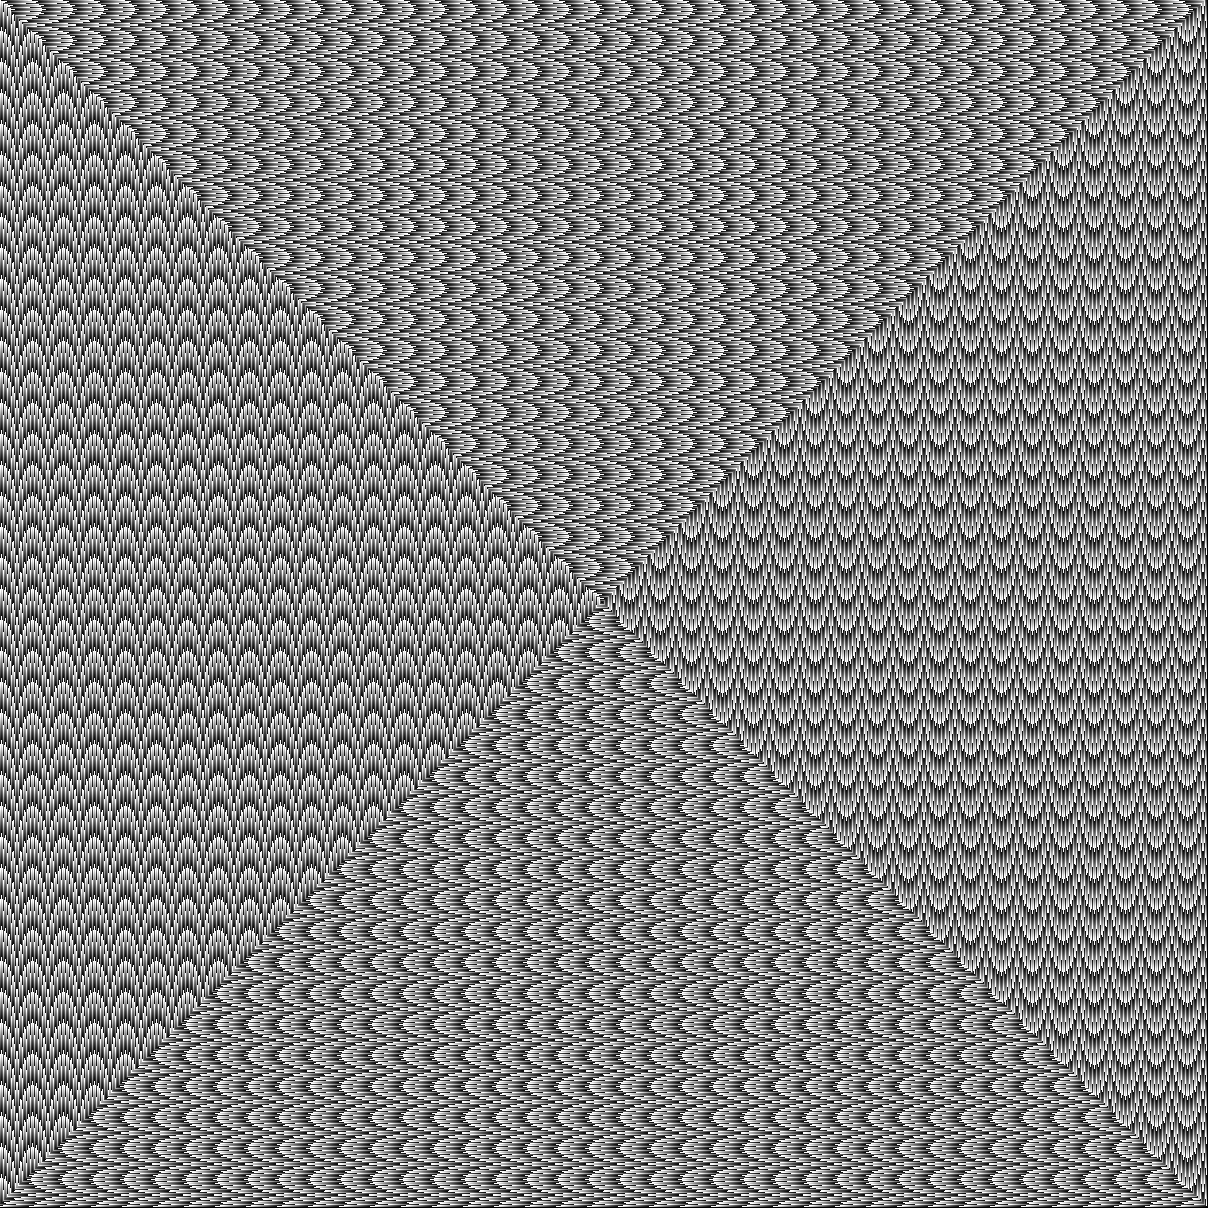
\includegraphics[scale=.3]{N31k39b.png}
\caption{Visualization of $Ond^{39}_{31}$}
\label{fig:viz3139}
\end{figure}

\begin{figure}[h]
\centering
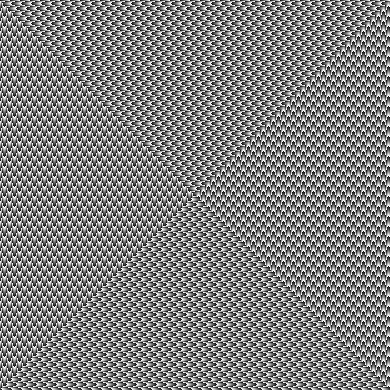
\includegraphics[scale=.9]{N10k39a.png}
\caption{Visualization of $Ond^{39}_{10}$}
\label{fig:viz1039}
\end{figure}


\end{document}  
